\pdfoutput=1
\documentclass[11pt]{article}
\usepackage[margin=1in]{geometry}
\usepackage{amsmath,amssymb,amsthm,booktabs,array}
\usepackage[shortlabels]{enumitem}
\usepackage[hidelinks]{hyperref}
\usepackage{algorithm}
\usepackage[noend]{algpseudocode}
\usepackage{tikz}
\usetikzlibrary{arrows.meta,backgrounds,calc,positioning,fit}
\tikzset{
  v/.style={circle,draw,fill=white,inner sep=0pt,minimum size=6pt,line width=0.6pt},
  d/.style={circle,fill=black,inner sep=0pt,minimum size=4.5pt},
  e/.style={line width=0.6pt},
  faint/.style={line width=0.5pt,black!30},
  arc/.style={line width=0.6pt,-{Stealth[length=4.5pt]}},
  lab/.style={font=\scriptsize},
  box/.style={draw,rounded corners=2pt,line width=0.6pt,align=center,font=\footnotesize,inner sep=4pt,minimum height=20pt},
  tool/.style={box,fill=black!6},
  main/.style={box,line width=1.1pt},
}


\setlist{itemsep=1pt,topsep=3pt}

\newtheorem{theorem}{Theorem}[section]
\newtheorem{lemma}[theorem]{Lemma}
\newtheorem{proposition}[theorem]{Proposition}
\theoremstyle{remark}
\newtheorem{remark}[theorem]{Remark}

\newcommand{\Ot}{\tilde O}
\newcommand{\AlgHold}{\textup{\textsc{Holding}}}
\newcommand{\AlgTrim}{\textup{\textsc{Trim}}}
\newcommand{\AlgLearn}{\textup{\textsc{Learn}}}

\title{Quantum Query Complexity of Recognizing\\ Threshold Graphs, Chain Graphs and Nested Matrices}
\hypersetup{pdftitle={Quantum Query Complexity of Recognizing Threshold Graphs, Chain Graphs and Nested Matrices},pdfauthor={Sebastian Senge}}
\author{Sebastian Senge\\ Independent Researcher}
\date{}

\begin{document}
\maketitle

\begin{abstract}
We give explicit quantum algorithms that use entry queries to a binary matrix or to an adjacency matrix, built from entry reads and quantum search. Classically all these problems need quadratically many queries. Our results are these:
\begin{itemize}[leftmargin=1.5em]
\item A nested $a\times b$ matrix, with equal rows and columns allowed, can be learned with $O((a+b)\log^3(a+b))$ queries.
\item Deciding whether an $n\times n$ matrix is nested takes $\Ot(n)$ queries, and $\Omega(n)$ queries are necessary.
\item Deciding whether a graph on $n$ vertices is a threshold graph takes $O(n\log^4 n)$ queries, and $\Omega(n)$ queries are necessary.
\item Deciding whether a graph on $n$ vertices is a chain graph takes $\Ot(n)$ queries, and $\Omega(n)$ queries are necessary.
\end{itemize}
The bounds count queries on a noiseless model.
\end{abstract}

\section{Introduction}

A binary $a\times b$ matrix is \emph{nested} if its rows, as subsets of the columns, form a chain under inclusion. A graph is a \emph{threshold graph} if it can be built by repeatedly adding an isolated or a dominating vertex. Equivalently~\cite{CH77}, it has no \emph{alternating $4$-cycle}: vertices $a,b,c,d$ with edges $ab,cd$ and non-edges $ac,bd$. A \emph{chain graph} is a bipartite graph whose neighbourhoods on one side are nested, together with possibly isolated vertices.

A query returns one entry of the matrix. Reading all entries is the only classical option in the worst case. An all-zero matrix and a matrix with one hidden $1$ are both nested, so learning takes $\Omega(ab)$ randomized queries, and Section~\ref{sec:recognition} gives $\Omega(n^2)$ for recognition.

\begin{table}[h]
\centering
\small
\renewcommand{\arraystretch}{1.25}
\begin{tabular}{@{}llll@{}}
\toprule
Problem & Previous best bound & Our bound & Lower bound\\
\midrule
Learn a nested $a\times b$ matrix, ties allowed & $O(ab)$ & $O((a+b)\log^3(a+b))$ & $\Omega(n\log n)$ \cite{MSZ25}\\
Is $M$ nested? $a,b=\Theta(n)$ & $O(n^2)$ & $\Ot(n)$ & $\Omega(n)$\\
Is $G$ a threshold graph? & $O(n^2)$ & $O(n\log^4 n)$ & $\Omega(n)$\\
Is $G$ a chain graph? & $O(n^2)$ & $\Ot(n)$ & $\Omega(n)$\\
\bottomrule
\end{tabular}
\caption{Quantum query bounds. The learning lower bound is for $a=b=n$.}
\label{tab:results}
\end{table}

\paragraph{Earlier work.} Half graphs are the nested matrices whose rows are all distinct and whose columns are all distinct. For them, \cite{MSZ25} gives $\Theta(n\log n)$ randomized and $\Theta(n\log n)$ quantum queries, with a quicksort that compares rows by quantum search. So equal rows and columns are what make the classical problem cost $\Omega(ab)$. Learning a nested matrix is also the bipartite sorting problem of~\cite{GJ22}, which has a classical algorithm within $\log^3$ of instance-optimal. Our contribution is a quantum learner with ties allowed, and the three recognition theorems. To our knowledge these have not been stated before.

The certificate of a non-threshold graph has $4$ vertices. So the natural baseline is the $\Ot(n^{3/2})$ of the quantum walk method for constant-size subgraphs~\cite{MSS05}. That result is stated for non-induced copies and monotone properties, while an alternating $4$-cycle uses non-edges. We compare against it nevertheless: against this baseline our gain is a factor of about $\sqrt n$, and against reading the input it is a factor of about $n$.

\paragraph{Technique.} A search over an $a\times b$ block costs $\sqrt{ab}\le(a+b)/2$ queries, up to the error term. A random pivot row and a random pivot column split a nested block into three blocks that, after trimming constant rows and columns, are disjoint in rows and in columns. So the cost per level of the recursion is linear.

\paragraph{Scope.} All bounds count queries. Section~\ref{sec:lean} states which parts are formalized in Lean. The other parts are claims with the proofs given here.

\section{Positions}

\begin{lemma}\label{lem:positions}
A matrix $M$ is nested if and only if there are integer positions $p$ on rows and $q$ on columns, with $p$ even and $q$ odd, such that $M[r,c]=1\iff p(r)>q(c)$.
\end{lemma}
\begin{proof}
Given positions, $N(r)=\{c:q(c)<p(r)\}$ grows with $p(r)$, so the rows are nested. Conversely let $S_0\subsetneq S_1\subsetneq\cdots$ be the distinct rows, and put $p(r)=2i$ for $N(r)=S_i$. Let $i(c)$ be the first $i$ with $c\in S_i$, or one more than the last index if $c$ is in no row, and put $q(c)=2i(c)-1$. Then $c\in N(r)\iff i(c)\le\mathrm{index}(r)\iff q(c)<p(r)$.
\end{proof}

So the columns of a nested matrix are nested too, and so is its complement.

\section{The learner}

A \emph{search} on $N$ candidates returns a uniformly random marked candidate, or none, in $O(\sqrt N\lambda)$ queries, with $\lambda=\log(1/\delta)$, and it wrongly reports none with probability at most $\delta$~\cite{BBHT98}.

\begin{algorithm}[h]
\caption{\AlgHold$(R,C,\mathit{val})$}
\begin{algorithmic}[1]
\State $K\gets\emptyset$
\Loop
  \State search $R\times(C\setminus K)$ for an entry equal to $\mathit{val}$
  \State \textbf{if} none \textbf{then return} $K$
  \State for the entry $(r,c)$ found, read row $r$ on $C$ and add its $\mathit{val}$-entries to $K$
\EndLoop
\end{algorithmic}
\end{algorithm}

\begin{lemma}\label{lem:holding}
On a nested block, with correct searches, \AlgHold{} returns exactly the columns that have an entry $\mathit{val}$, in $O(\log|R|)$ expected rounds.
\end{lemma}
\begin{proof}
The set is correct by the stopping rule. By Lemma~\ref{lem:positions} for $M$ or its complement, the sets $\{c:M[r,c]=\mathit{val}\}$ are nested. Let $U$ be the rows with an entry $\mathit{val}$ outside $K$. The number of such entries in $r\in U$ grows along the chain, so the upper half of $U$ holds at least half of the marked entries. With probability at least $1/2$ the row found is in the upper half. After reading it, $K$ contains all $\mathit{val}$-entries of every row at or below it in the chain, so $|U|$ at least halves.
\end{proof}

\paragraph{Trimming.} The call \AlgTrim$(R,C)$ works as follows. Run \AlgHold{} on columns and, on the transpose, on rows, for $\mathit{val}=0$ and $\mathit{val}=1$, all on this same block. A row or column missing from the list for $\mathit{val}$ is constant $1-\mathit{val}$ on the block. Record those entries and remove it. Removal is one pass, relative to the block given.

\begin{algorithm}[h]
\caption{\AlgLearn$(R,C)$}
\begin{algorithmic}[1]
\If{$|R||C|\le 4(|R|+|C|)$} read all entries and \Return \EndIf
\State pick $x\in R$ and $w\in C$ uniformly at random
\State read row $x$ on $C$, giving $C_1$ (its $1$-entries) and $C_0$
\State read column $w$ on $R$, giving $R_1$ (its $1$-entries) and $R_0$
\If{$M[x,w]=1$}
  \State record $R_0\times C_0$ as $0$; let $\mathcal B=\{R_0\times C_1,\ R_1\times C_1,\ R_1\times C_0\}$
\Else
  \State record $R_1\times C_1$ as $1$; let $\mathcal B=\{R_0\times C_1,\ R_0\times C_0,\ R_1\times C_0\}$
\EndIf
\State for each $B\in\mathcal B$, run \AlgLearn$(\AlgTrim(B))$
\end{algorithmic}
\end{algorithm}

\begin{figure}[t]
\centering
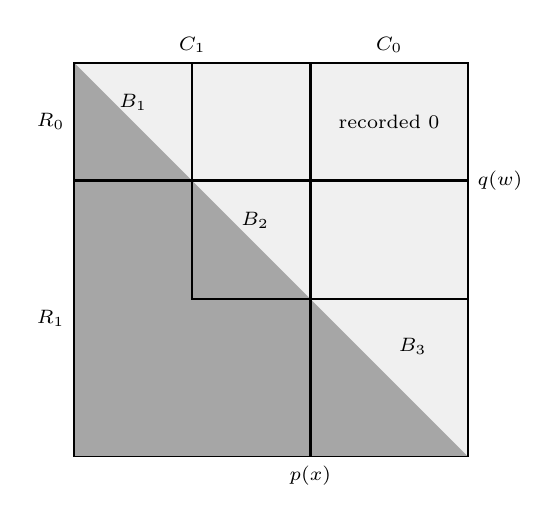
\begin{tikzpicture}[x=0.5cm,y=-0.5cm]
  % positions grow to the right (columns) and downwards (rows); an entry is 1 iff p(r) > q(c)
  \fill[black!6] (0,0) -- (10,0) -- (10,10) -- cycle;
  \fill[black!35] (0,0) -- (0,10) -- (10,10) -- cycle;
  \draw[e] (0,0) rectangle (3,3);
  \draw[e] (3,3) rectangle (6,6);
  \draw[e] (6,6) rectangle (10,10);
  \draw[e] (0,0) rectangle (10,10);
  \draw[line width=1pt] (0,3) -- (10,3);
  \draw[line width=1pt] (6,0) -- (6,10);
  \node[lab,left] at (0,1.5) {$R_0$};
  \node[lab,left] at (0,6.5) {$R_1$};
  \node[lab,above] at (3,0) {$C_1$};
  \node[lab,above] at (8,0) {$C_0$};
  \node[lab] at (8,1.5) {recorded $0$};
  \node[lab] at (1.5,1.0) {$B_1$};
  \node[lab] at (4.6,4.0) {$B_2$};
  \node[lab] at (8.6,7.2) {$B_3$};
  \node[lab,right] at (10,3) {$q(w)$};
  \node[lab,below] at (6,10) {$p(x)$};
\end{tikzpicture}

\caption{A split in the case $M[x,w]=1$. Rows and columns are sorted by position, although the algorithm does not know this order. Dark entries are $1$ and light entries are $0$. Trimming removes the constant rows and columns of each block, and the blocks $B_1,B_2,B_3$ remain.}
\label{fig:split}
\end{figure}

\begin{lemma}[Exact split]\label{lem:split}
On a nested block, the recorded entries are right, and the three trimmed blocks are contained in three disjoint position intervals. So every row and every column survives into at most one of them.
\end{lemma}
\begin{proof}
Write $p=p(x)$ and $q=q(w)$. Then $R_0=\{r:p(r)<q\}$, $R_1=\{r:p(r)>q\}$, $C_1=\{c:q(c)<p\}$ and $C_0=\{c:q(c)>p\}$.

\emph{Case $q<p$, so $M[x,w]=1$.} On $R_0\times C_0$ we have $p(r)<q<p<q(c)$, which gives $0$.
\begin{itemize}[leftmargin=1.5em]
\item $R_0\times C_1$: a column with $q(c)\ge q$ lies above all rows of $R_0$, so it is constant $0$ and is trimmed. What survives lies below $q$.
\item $R_1\times C_1$: a row with $p(r)\ge p$ lies above all columns of $C_1$, so it is constant $1$. A column with $q(c)\le q$ lies below all rows of $R_1$, so it is constant $1$. What survives lies strictly between $q$ and $p$.
\item $R_1\times C_0$: a row with $p(r)\le p$ lies below all columns of $C_0$, so it is constant $0$. What survives lies above $p$.
\end{itemize}

\emph{Case $p<q$, so $M[x,w]=0$.} On $R_1\times C_1$ we have $p(r)>q>p>q(c)$, which gives $1$.
\begin{itemize}[leftmargin=1.5em]
\item $R_0\times C_1$: a row with $p(r)\ge p$ is constant $1$. What survives lies below $p$.
\item $R_0\times C_0$: a row with $p(r)\le p$ is constant $0$, and a column with $q(c)\ge q$ is constant $0$. What survives lies strictly between $p$ and $q$.
\item $R_1\times C_0$: a column with $q(c)\le q$ is constant $1$. What survives lies above $q$.\qedhere
\end{itemize}
\end{proof}

\begin{lemma}[Balance]\label{lem:balance}
Let $m=|R|+|C|$. With probability at least $1/4$, each trimmed block has at most $3m/4$ rows and columns.
\end{lemma}
\begin{proof}
Let $a=|R|$ and $b=|C|$, and order the rows by $p$, breaking ties arbitrarily. A row of rank $i$ has at most $i-1$ rows strictly below it and at most $a-i$ strictly above. Both are at most $3a/4$ for $a/4\le i\le 3a/4+1$, which covers at least $a/2$ ranks. So $x$ has this property with probability at least $1/2$, and independently $w$ has the same property with $3b/4$. By Lemma~\ref{lem:split}, the surviving rows of a block lie strictly on one side of $p(x)$, and its surviving columns strictly on one side of $q(w)$. So each block has at most $3a/4+3b/4$ rows and columns.
\end{proof}

\begin{theorem}\label{thm:learn}
\AlgLearn{} determines a nested $a\times b$ matrix with $O((a+b)\log^3(a+b))$ expected queries and bounded error. For $a=b=n$, at least $\Omega(n\log n)$ quantum queries are necessary~\cite{MSZ25}, and classically $\Omega(ab)$ randomized queries are necessary.
\end{theorem}
\begin{proof}
Correctness follows from Lemmas~\ref{lem:holding} and~\ref{lem:split} by induction. For the cost, a node with $m$ rows and columns reads $m$ entries and makes four calls to \AlgHold{} per block. By Lemma~\ref{lem:holding} each call has $O(\log m)$ expected rounds, and each round costs a search at $O(m\lambda)$ queries and a read of $m$ entries. By Lemma~\ref{lem:split} the blocks at one depth are disjoint in rows and in columns, and by Lemma~\ref{lem:balance} a given row or column lies in $O(\log m)$ levels in expectation. So the expected total is $O(m\log^2 m\cdot\lambda)$. Base cases read at most $4$ entries per row or column. There are polynomially many searches, so $\lambda=O(\log m)$ gives error $1/10$ by a union bound. Truncating at ten times the expected cost adds error $1/10$ and makes the bound hold in the worst case.

The classical bound follows from the all-zero matrix against a single hidden $1$.
\end{proof}

Only the lists of Lemma~\ref{lem:holding} use the uniform outcome of the search.

\section{Recognition}\label{sec:recognition}

\paragraph{Check.} Learn a hypothesis $H$, and reject if the learner was truncated or if $H$ is not in the class, which costs no queries. Then search all entries for a disagreement with the input, at $O(\sqrt{ab})$ queries. If the input is in the class, then $H$ equals it with high probability, and the answer is yes. If it is not, then $H$ differs from the input, since $H$ is in the class, and the search finds a disagreement with high probability. So correctness does not depend on what the learner does on inputs outside the class.

\paragraph{Hard family.} Let the vertices $0,\dots,n-1$ have the creation sequence $0,1,0,1,\dots$, so that an odd vertex $j$ is adjacent to all $i<j$. For even $i$ and odd $j\ge i+3$, delete the edge $ij$. Then $j,i+2,i+1,i$ is an alternating $4$-cycle, since $j\sim i+2$ and $i+1\sim i$, while $j\not\sim i$ and $i+1\not\sim i+2$. There are $\Theta(n^2)$ such pairs. So deciding the class on inputs with no deletion or one deletion is an OR on $\Theta(n^2)$ bits with at most one $1$, which needs $\Omega(n)$ quantum and $\Omega(n^2)$ randomized queries. The bipartite part between odd and even vertices gives the same for nested matrices and for chain graphs.

\begin{theorem}\label{thm:nested}
Deciding whether an $a\times b$ matrix is nested takes $\Ot(a+b)$ quantum queries, and $\Omega(\sqrt{ab})$ queries are necessary on matrices of the shapes of the hard family. So the bound is tight up to logarithmic factors for $a=\Theta(b)$.
\end{theorem}

\begin{theorem}\label{thm:threshold}
Deciding whether a graph on $n$ vertices is a threshold graph takes $O(n\log^4 n)$ quantum queries. At least $\Omega(n)$ quantum queries and $\Omega(n^2)$ randomized queries are necessary.
\end{theorem}
\begin{proof}
Split the vertices in two parts $A,B$. If $G$ is a threshold graph, then the cross block $A\times B$ has no $2\times2$ permutation pattern, since that would be an alternating $4$-cycle, so it is nested. Learn it, and recurse on $A$ and on $B$. Each pair of vertices falls in exactly one block, and the split avoids the diagonal of the adjacency matrix, on which no query is defined. The recurrence $L(n)=2L(n/2)+O(n\log^3 n)$ gives $O(n\log^4 n)$. All searches share one $\lambda=O(\log n)$ and the whole run shares one truncation, so the error of Theorem~\ref{thm:learn} is not paid $n$ times. The check costs $O(n)$. The lower bounds come from the hard family.
\end{proof}

\begin{theorem}\label{thm:chain}
Deciding whether a graph on $n$ vertices is a chain graph takes $\Ot(n)$ quantum queries. At least $\Omega(n)$ quantum queries and $\Omega(n^2)$ randomized queries are necessary.
\end{theorem}
\begin{proof}
Search for an edge $(x,y)$. If none exists, accept. Read $X:=N(y)$. With \AlgHold{} on rows $X$ and all vertices, compute $Y:=N(X)$. With \AlgHold{} again, compute $X:=N(Y)$. In a chain graph with sides $A\ni x$ and $B\ni y$, the set $N(y)$ contains the top vertex $a^*$ of $A$, since $a^*$ is adjacent to all non-isolated vertices of $B$. So $Y\supseteq N(a^*)$ is the set of all non-isolated vertices of $B$, and likewise the second step gives all non-isolated vertices of $A$. Reject if $X\cap Y\ne\emptyset$. Learn $X\times Y$, and check against the input on all pairs.
\end{proof}

\begin{proposition}\label{prop:matchings}
Learning any class of graphs that contains all perfect matchings takes $\Omega(n^{3/2})$ quantum queries~\cite{MSZ25}. This includes cographs, trivially perfect graphs, unit interval graphs, interval graphs, permutation graphs and distance-hereditary graphs.
\end{proposition}

So the bound of Theorem~\ref{thm:learn} depends on the absence of a $2\times 2$ permutation pattern in cross blocks. Recognition does not have to go through learning, and for those classes it is open.

\section{Simulation and circuits}\label{sec:sim}

The repository has simulation scripts, in which a search is sampled from the exact outcome law of quantum search with a budget per search, and a circuit test.
\begin{itemize}[leftmargin=1.5em]
\item On all $33{,}867$ graphs with up to $6$ vertices, for threshold and chain graphs, there is no wrong answer against an independent classical decision. Families and single flips agree up to $n=150$.
\item At a budget of $16$ per search and $n=1024$, the recognizer spends about $454{,}000$ queries on yes inputs, against $523{,}776$ entries for reading all pairs. At $n=2048$, it spends about $1.2$ million queries against $2.1$ million entries on the worst family run.
\item A budget of $16$ gives $1$ wrong answer in $300$ at $n=1024$, and none in $80$ at $n=2048$. A constant budget cannot hold for all $n$, since the proof needs $\lambda=\Theta(\log n)$.
\item Fitted exponents at $n\le 2048$ are $1.0$ to $1.4$.
\item With every search a circuit in Qiskit, on at most $8$ qubits, $30$ runs give no wrong answer. At these sizes the algorithm spends far more queries than there are entries, so this tests the construction and shows no gain.
\end{itemize}
Inputs far from the class can cost far more than reading everything. A practical version stops at the cost of reading everything and then reads everything, so it never pays more than twice the classical cost.

\section{Formal verification}\label{sec:lean}

The Lean files in the repository build with no \texttt{sorry}, and \texttt{\#print axioms} reports only the standard axioms.

\paragraph{Proved.} Lemma~\ref{lem:positions}. Lemma~\ref{lem:split}. Lemma~\ref{lem:balance}. Correctness of \AlgHold, \AlgTrim{} and \AlgLearn, given correct searches and enough fuel. The round bound of Lemma~\ref{lem:holding}, given uniform search. Correctness of the check and of the three recognizers, given correct searches. The characterization of threshold graphs by alternating $4$-cycles, and the nesting of cross blocks. The hard family. The expected cost as accounting, for Theorems~\ref{thm:learn} and~\ref{thm:threshold}.

\paragraph{Stated as hypotheses.} The cost and law of quantum search, and the OR lower bound, on an explicit query model.

\paragraph{Not formalized.} Queries are not counted from an execution, since the learner is a classical function and its cost is accounting. Pivot and search randomness are not combined in one space. The union bound over searches and the truncation are absent, so bounded error and the worst-case forms of the theorems are not covered. Also absent are the classical lower bounds, the learning lower bound, a cost theorem for the chain recognizer, and Proposition~\ref{prop:matchings}.

\section{Open questions}

\begin{itemize}[leftmargin=1.5em]
\item The power of the logarithm. The learner has $\Omega(n\log n)$ and $O(n\log^3 n)$. Runs suggest that one logarithm in the analysis may not be needed.
\item Recognition of cographs and of trivially perfect graphs. Their certificates have constant size, so adversary methods stop at $O(n)$.
\item Unbalanced shapes of Theorem~\ref{thm:nested}. For $a=2$ this is subset testing, at $\Theta(\sqrt b)$ queries, while the learner reads $b$ entries.
\end{itemize}

\section*{Use of AI}

The proofs, the code and the Lean files were developed with Claude Opus~5.5 (Anthropic), which was also used to search the literature, to review the proofs and to draft the text.

\begin{thebibliography}{99}
\bibitem{BBHT98} M.~Boyer, G.~Brassard, P.~H\o yer, A.~Tapp. Tight bounds on quantum searching. Fortschritte der Physik 46, 1998, arXiv:quant-ph/9605034.
\bibitem{CH77} V.~Chv\'atal, P.~Hammer. Aggregation of inequalities in integer programming. Annals of Discrete Mathematics 1, 1977.
\bibitem{GJ22} M.~Goswami, R.~Jacob. On instance-optimal algorithms for a generalization of nuts and bolts and generalized sorting. arXiv:2211.04601.
\bibitem{MSS05} F.~Magniez, M.~Santha, M.~Szegedy. Quantum algorithms for the triangle problem. SODA 2005, arXiv:quant-ph/0310134.
\bibitem{MSZ25} N.~S.~Mande, S.~Sanyal, V.~Zamaraev. Complexity of learning matchings and half graphs via edge queries. arXiv:2507.03151.
\end{thebibliography}

\end{document}
